\documentclass{article}
\usepackage[utf8]{inputenc}
\usepackage{graphicx}

\author{Bijan Varjavand}
\title{LabNotebook}
\date{March 7, 2017}

\begin{document}

\maketitle

\section{Objectives}

This lab had 2 different tasks, the first was to visually see the differences in index of refraction between a solid and liquid by how visible the interface was.\\
The other objective was to understand total internal reflection in waveguides.

\section{Setup}

Wires and breadboards were provided, as well as waveguides and LEDs. We were also given the necessary reagents and materials to prepare the index of refraction part of the lab.

\subsection{Materials}

We used borosilicate, polyacrylamide, polystyrene, and water for the first part.\\

The second part utilized waveguides and other plastic tubing.

\subsection{Tools}

The main tools used were power supply, ammeter, and voltmeter for the seconds part.

\section{Procedure}

My group wast the first to do the visual refractive index lab, so we had to aliquot out all the chemicals. After, we dropped the different materials into each solvent and qualitatively measured how clearly we could see them.\\

The second part of the lab is more involved - we had to measure the amount of light emitted from the end of a waveguide with different waveguides and different light wavelengths.

\section{Results}

Results of our experiments are shown below

\begin{figure}[h!]
\centering
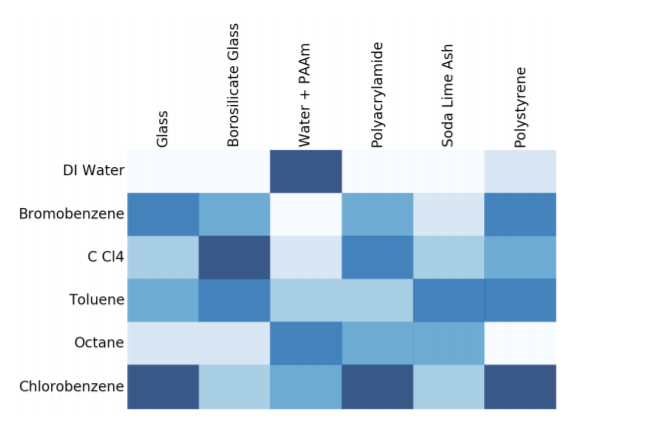
\includegraphics[scale=0.6]{refract.png}
\end{figure}

\begin{figure}[h!]
\centering
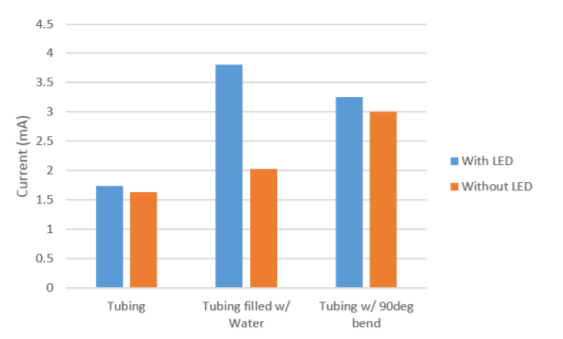
\includegraphics[scale=0.8]{lights.png}
\end{figure}

\begin{figure}[h!]
\centering
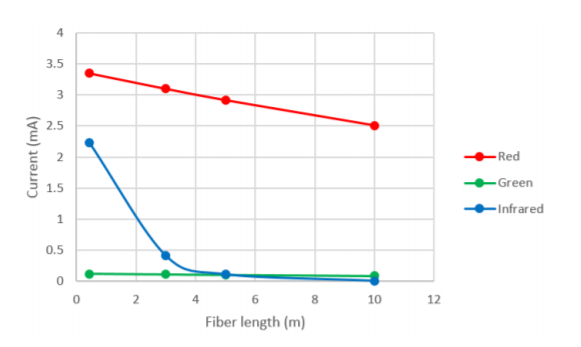
\includegraphics[scale=0.8]{wave.png}
\end{figure}

\section{Observations}

It seemed clear that, after looking up the indices of refraction of each material, that the material and solvent with similar refractive indices seemed to merge. The material became less visible.\\
The plastic waveguides didn't properly contain the light with a 90 degree bend. Also, adding water improved waveguide performance. It was also seen that the amount of loss each waveguide exhibited depended on the wavelength of light used.

\end{document}